\section{Contemporary observed-data case studies}\label{sec:updated-case-studies}

\subsection{Data sources and scientific scope}
We replace the archived 1990--1999 carbon-dioxide demonstration in
the submission with a frozen 441-month sequence of directly
published NOAA Global Monitoring Laboratory (GML) Mauna Loa
monthly-mean atmospheric $\mathrm{CO}_2$ concentrations,
January 1990--September 2026, in parts per million
\cite{noaa2026mlo}. The September 2026 observation is
426.07 ppm; October 2026 is not included because a complete
monthly value had not been released at the October 26 data cutoff.
The source snapshot and provenance accompany the submission.
Unlike the earlier \texttt{statsmodels} historical example, these
are published monthly observations rather than calendar-month
averages constructed from an archived weekly file.
The strong seasonal cycle remains in the data; it should not be
conflated with observational error or removed implicitly by PLS.
We also study the most recent 120-month subset of this record to
isolate the consequences of a shorter estimation window.

For an independent economic example, we use the US effective federal funds rate (FEDFUNDS), the
monthly average of daily rates (not seasonally adjusted), from January 2010 through September 2026 ($n=201$).
The underlying source is the Board of Governors of the Federal Reserve System
and the distribution is through the Federal Reserve Economic
Data (FRED) service \cite{fred2026fedfunds}. The September 2026
release reports 3.75 percent. The snapshot is retained with its
download URL, last observation, checksum, and retrieval procedure.
Both records may subsequently be revised by their publishers.

\subsection{Four selectors, two parameterizations, four orders}
For each series and $d\in\{1,2,3,4\}$ we fix $\mu=0$ and compare
CV, GCV, AICc, BIC, and the controlled normalized smoothness
$S=0.86$. For the four score-based selectors we use a common
29-point interior smoothness grid
$\mathcal S=\{0.10,0.10+0.88/28,\ldots,0.98\}$.
Each candidate $s$ is mapped to its unique penalty
$\lambda=S^{-1}(s)$, and all four criteria are evaluated on the
\emph{same} resulting penalty candidates. Thus differences in
the selected fitted curves are attributable to the criterion
at a given $d$, rather than differing numerical search domains.
The controlled-$S$ fit is an explicit user choice, not a
fifth automatically optimized criterion.

The experiment records both $\widehat\lambda$ and
$\widehat S=S(\widehat\lambda)$ for every selected fit.
These are two coordinates for one smoother, not two
independent estimators. When comparing $d$ values,
a common $S$ equalizes the fraction of penalizable trace
degrees of freedom, not the space of admissible
polynomial components. In particular $\dim\ker(D_d)=d$,
and higher orders may have less stable endpoint behavior.

\begin{figure}[tbp]
\centering
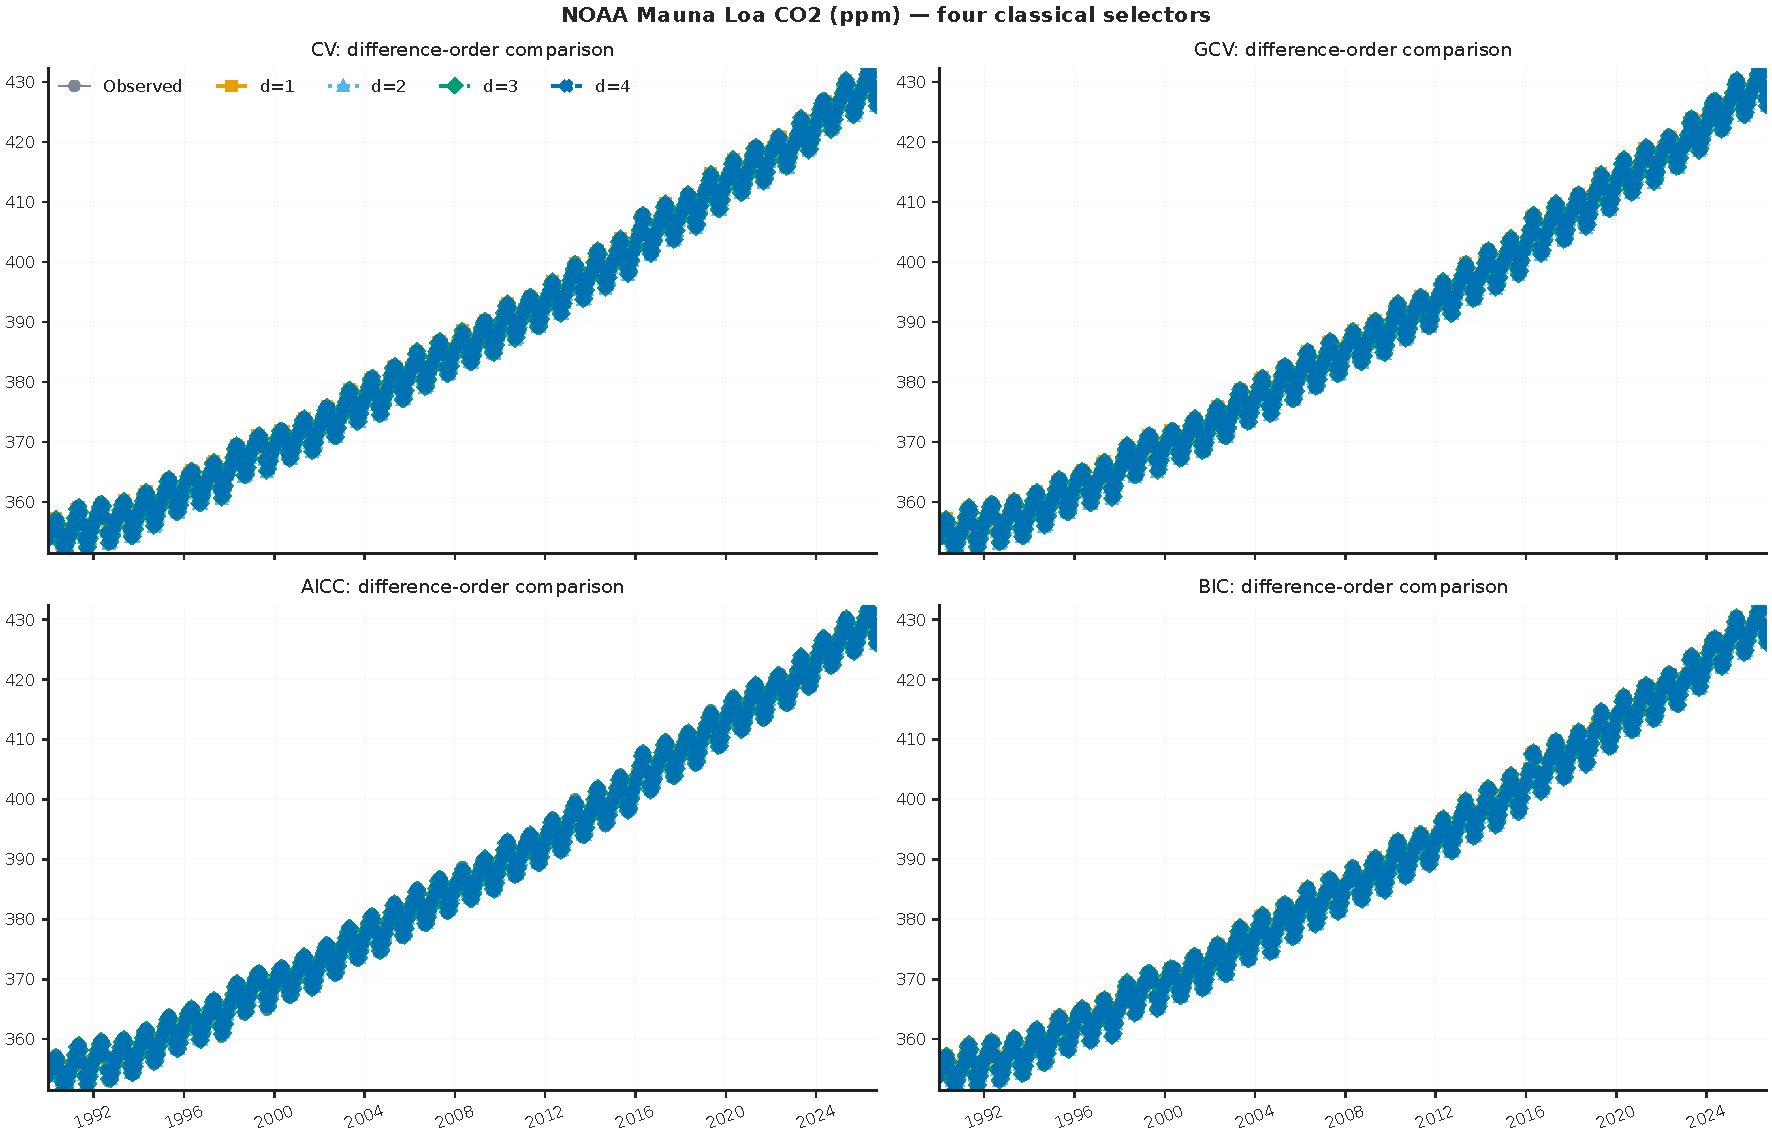
\includegraphics[width=\linewidth]{figures/co2_full_criteria.pdf}
\caption{Four classical criterion choices applied to NOAA
Mauna Loa monthly mean CO$_2$, 1990--September 2026,
at difference orders $d=1,2,3,4$ and fixed $\mu=0$.
All panels use identical candidate-$S$ grids within each
order. These are in-sample two-sided trends, not forecasts.}
\label{fig:co2-current-criteria}
\end{figure}

\begin{figure}[tbp]
\centering
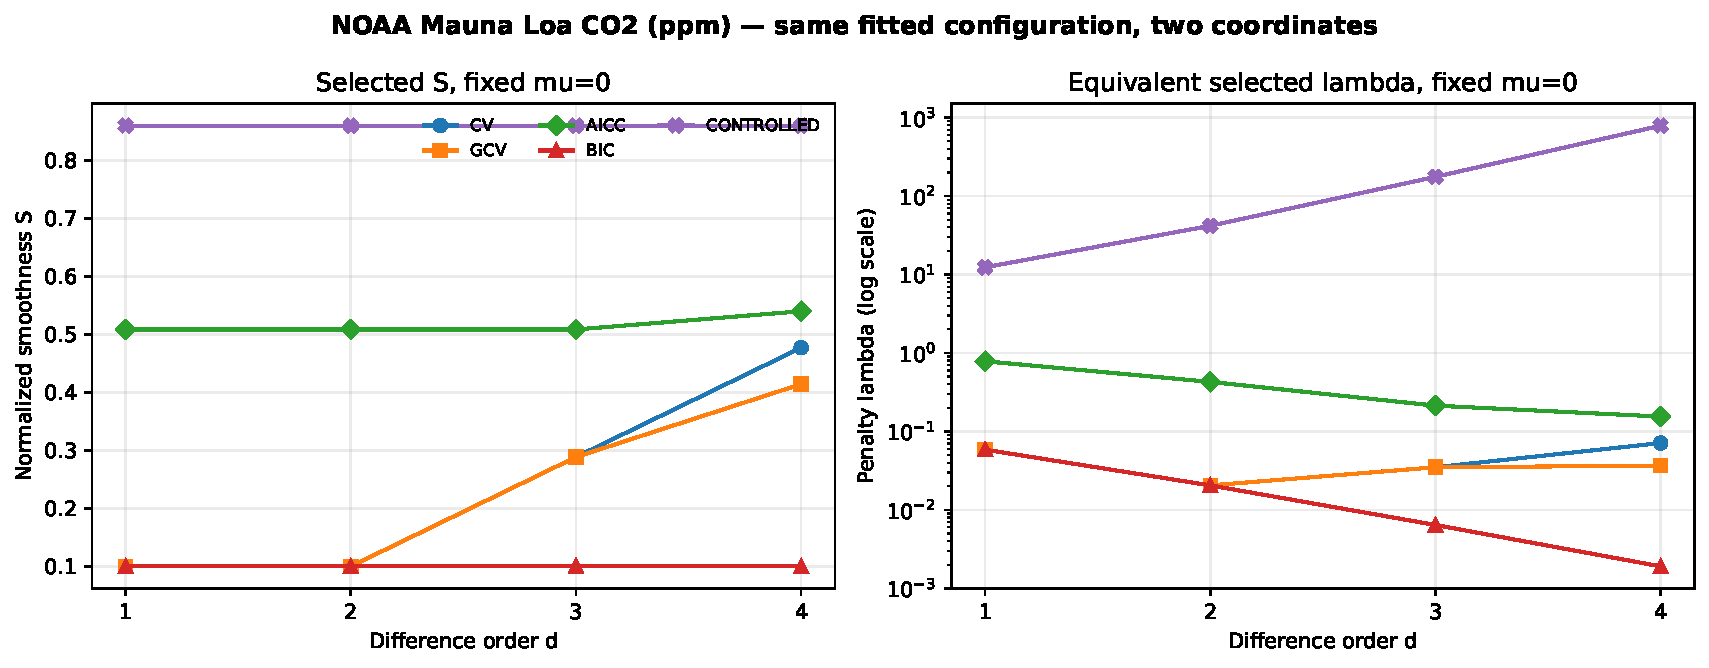
\includegraphics[width=.96\linewidth]{figures/co2_full_selected_coordinates.pdf}
\caption{The identical CO$_2$ selections reported as normalized
smoothness $S(\widehat\lambda)$ (left) and penalty
$\widehat\lambda$ (right). The controlled value $S=0.86$
is the prescribed point across orders; the other points
minimize their named scores over the candidate grid.}
\label{fig:co2-selection-coordinates}
\end{figure}

\begin{figure}[tbp]
\centering
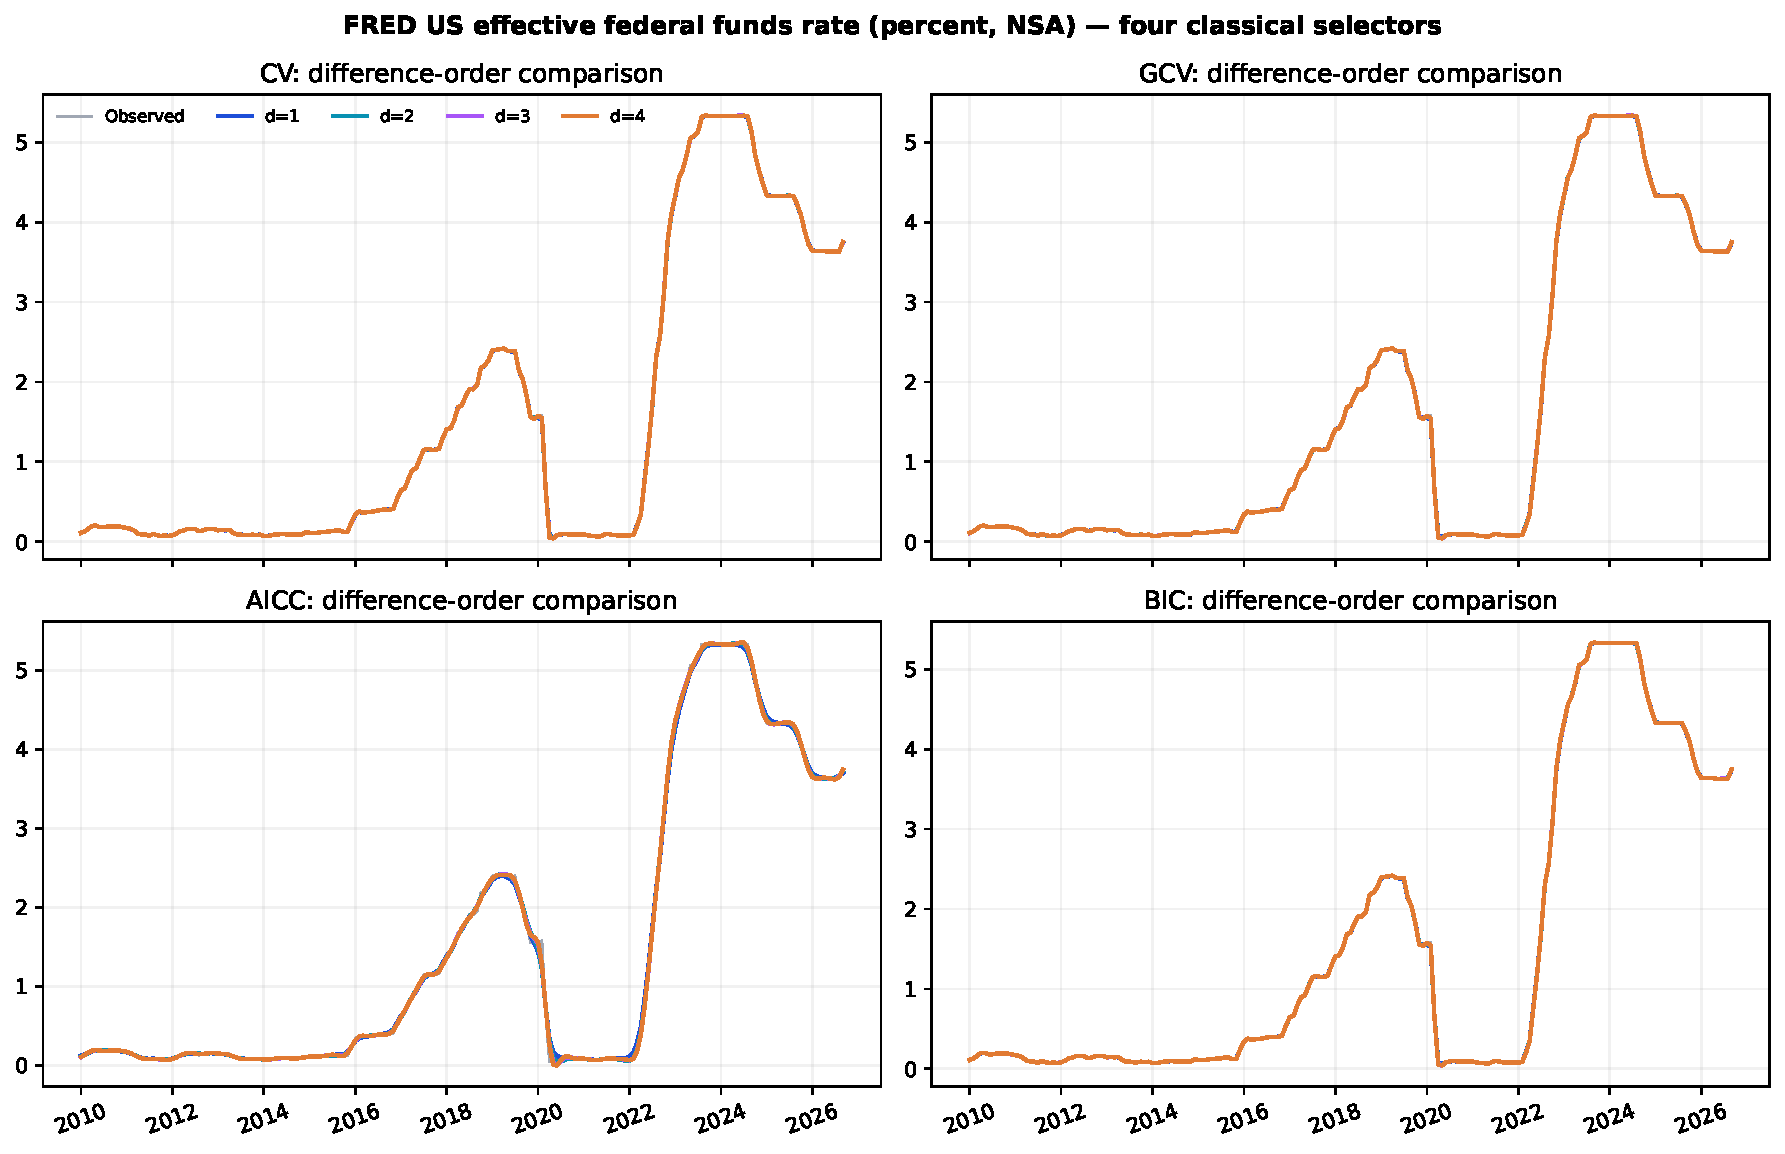
\includegraphics[width=\linewidth]{figures/fedfunds_full_criteria.pdf}
\caption{US monthly not not monthly effective federal funds rate
(FEDFUNDS), January 2010--September 2026,
with CV, GCV, AICc, and BIC selections across
$d=1,2,3,4$. This independent macroeconomic example
illustrates structurally different dynamics from the
seasonally varying CO$_2$ record.}
\label{fig:fedfunds-current-criteria}
\end{figure}

\begin{table}[tbp]
\centering
\caption{Reproducibly selected penalties, normalized
smoothness and 12-month single-origin holdout RMSE
for $d=2$ across the full CO$_2$ record, its last
120 months, and not monthly effective federal funds rate.
The controlled smoothness $S=0.86$ is prescribed.
CO$_2$ errors are in ppm and federal funds rate errors
in percentage points; the RMSE values are \emph{not}
directly comparable across datasets. The 12-month
evaluation is exploratory, not a rolling-origin
performance estimate.}
\label{tab:current-examples}
\footnotesize
\begin{tabular}{llrrr}\toprule
Dataset & Selector & $\lambda$ & $S$ & holdout RMSE\\\midrule
CO$_2$ (1990--2026) & CV & 0.02055 & 0.100 & 2.597\\
CO$_2$ (1990--2026) & GCV & 0.02055 & 0.100 & 2.597\\
CO$_2$ (1990--2026) & AICC & 0.4284 & 0.509 & 2.596\\
CO$_2$ (1990--2026) & BIC & 0.02055 & 0.100 & 2.597\\
CO$_2$ (1990--2026) & CONTROLLED & 41.77 & 0.860 & 2.520\\
CO$_2$ (recent 120 months) & CV & 0.02053 & 0.100 & 2.597\\
CO$_2$ (recent 120 months) & GCV & 0.02053 & 0.100 & 2.597\\
CO$_2$ (recent 120 months) & AICC & 0.4234 & 0.509 & 2.596\\
CO$_2$ (recent 120 months) & BIC & 0.02053 & 0.100 & 2.597\\
CO$_2$ (recent 120 months) & CONTROLLED & 37.03 & 0.860 & 2.524\\
Fed funds (2010--2026) & CV & 0.02054 & 0.100 & 1.009\\
Fed funds (2010--2026) & GCV & 0.02054 & 0.100 & 1.009\\
Fed funds (2010--2026) & AICC & 1.212 & 0.634 & 1.012\\
Fed funds (2010--2026) & BIC & 0.02054 & 0.100 & 1.009\\
Fed funds (2010--2026) & CONTROLLED & 39.57 & 0.860 & 1.067\\
\bottomrule\end{tabular}

\end{table}

\subsection{Future extension versus validated forecasting}
The fitted trend is only defined at observed time indices.
To illustrate possible trajectories \emph{without attributing
a forecasting model to the PLS smoother}, we regress the
final 36 fitted values on a locally centered polynomial
of degree $\min(d-1,2)$ and evaluate that polynomial for
the next 12 months, October 2026--September 2027.
For $d=1$ this is a constant continuation, $d=2$ a
linear continuation, and $d\ge3$ a quadratic continuation.
The degree cap is an explicitly imposed stability choice:
an unrestricted degree-$d-1$ extrapolation for large $d$
can diverge rapidly. These lines extrapolate the
\emph{smoothed trend only}; they do not forecast
CO$_2$ seasonal components, policy shocks, or
interest-rate policy changes, and no predictive intervals
are inferred.

\begin{figure}[tbp]
\centering
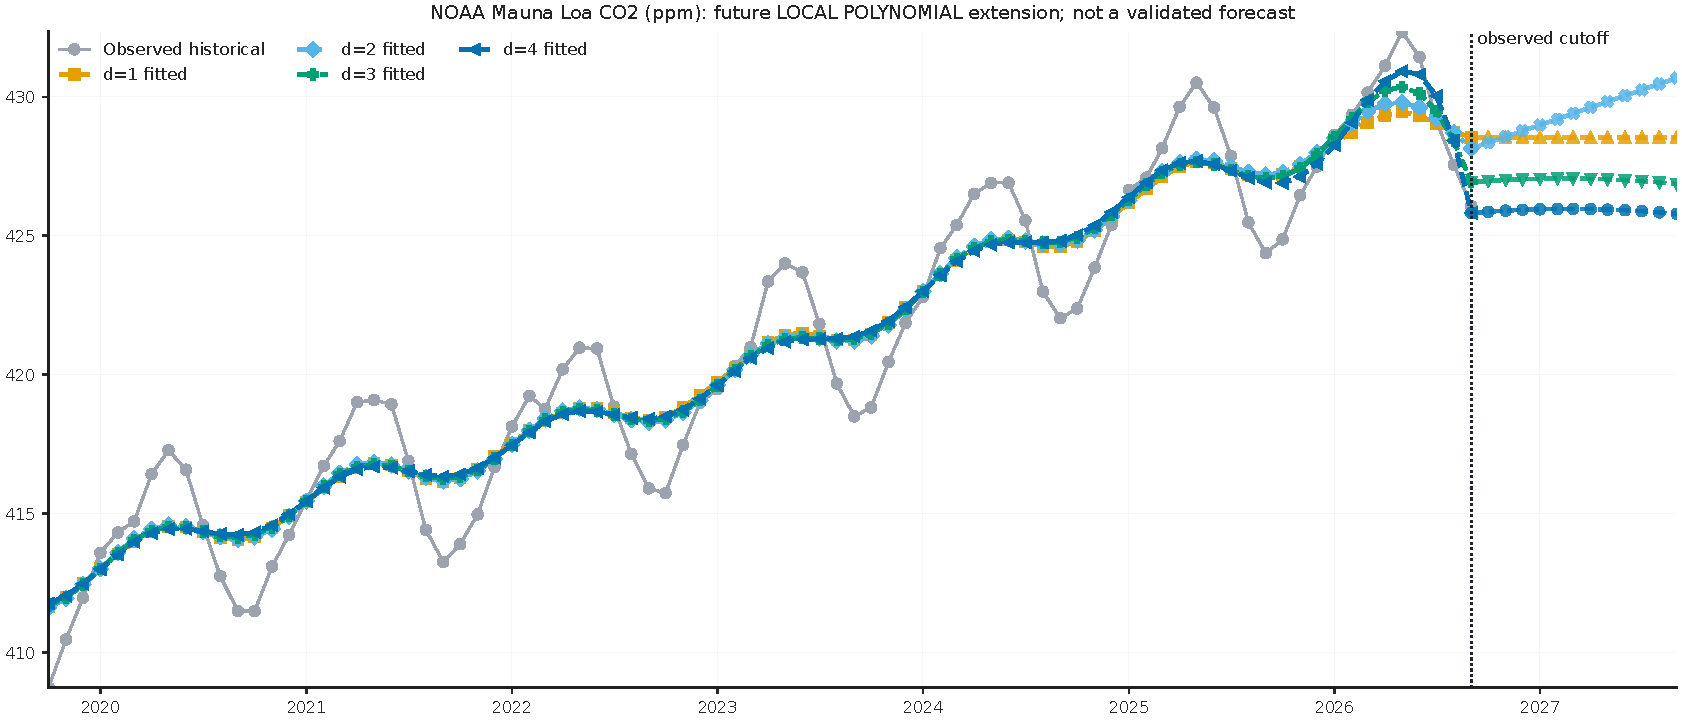
\includegraphics[width=\linewidth]{figures/co2_full_future_extrapolations.pdf}
\caption{Descriptive trend extension from all NOAA observations
through September 2026 (vertical cutoff) to the subsequent
12 calendar months. Solid lines are fitted trends with
common $S=0.86$; dashed lines are local-polynomial
\emph{extrapolations}. They are not observed future data,
model-based forecasts, or confidence intervals.}
\label{fig:co2-extrapolation}
\end{figure}

\begin{figure}[tbp]
\centering
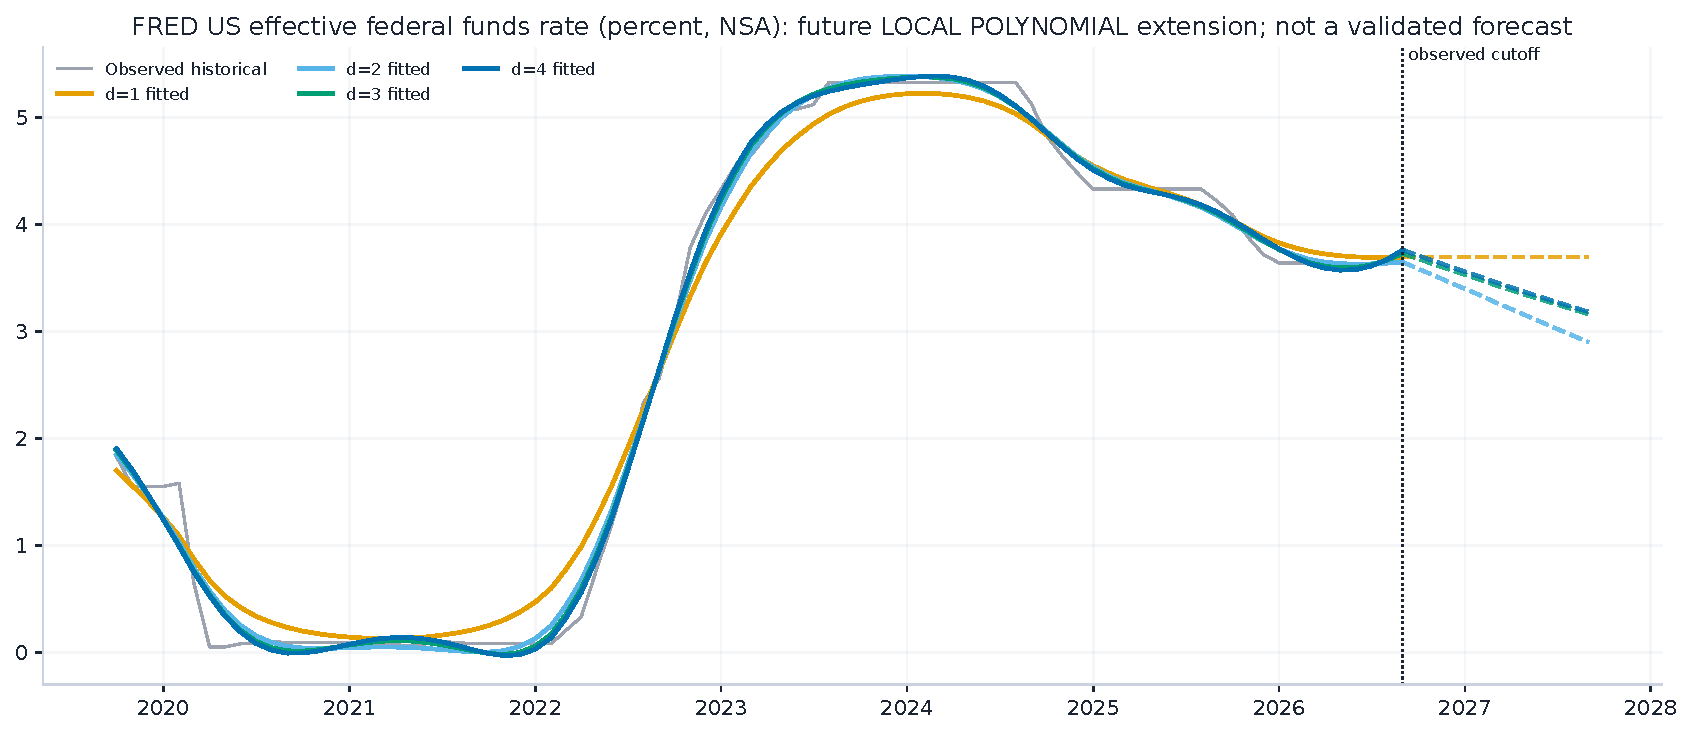
\includegraphics[width=\linewidth]{figures/fedfunds_full_future_extrapolations.pdf}
\caption{Corresponding trend-only 12-month extension for
not monthly federal funds effective rate. The different
orders may imply substantially different extrapolation
slopes or curvature even at identical normalized $S$.
Dashed segments are illustrative, not validated forecasts.}
\label{fig:fedfunds-extrapolation}
\end{figure}

As an independent \emph{single-origin diagnostic}, we additionally
stop estimation 12 months before the published end date,
choose the criterion and compute the fit using that training
segment alone, and compare 12-step extrapolations with the
held-out subsequent observations. This avoids look-ahead
leakage from the test period. It is not a substitute for
multiple rolling forecast origins, uncertainty calibration,
or explicit seasonal models.

\begin{figure}[tbp]
\centering
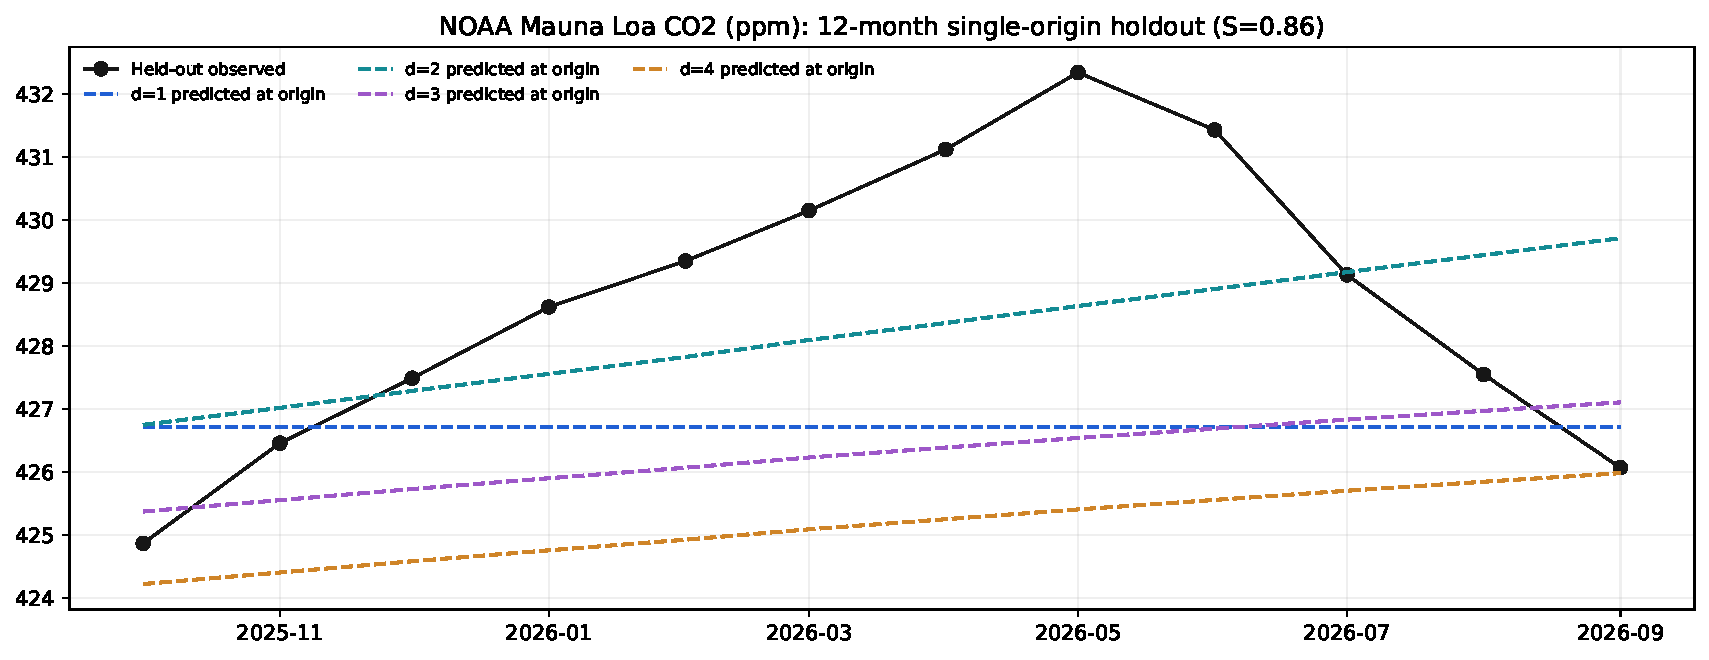
\includegraphics[width=\linewidth]{figures/co2_full_heldout_backtest.pdf}
\caption{Historical 12-month holdout observations and trend-only
extrapolations made from the preceding training segment,
using controlled $S=0.86$. CO$_2$ seasonal fluctuations
remain in the observations; poor agreement cannot be
interpreted as a clean test of trend extraction alone.}
\label{fig:co2-holdout}
\end{figure}

\begin{figure}[tbp]
\centering
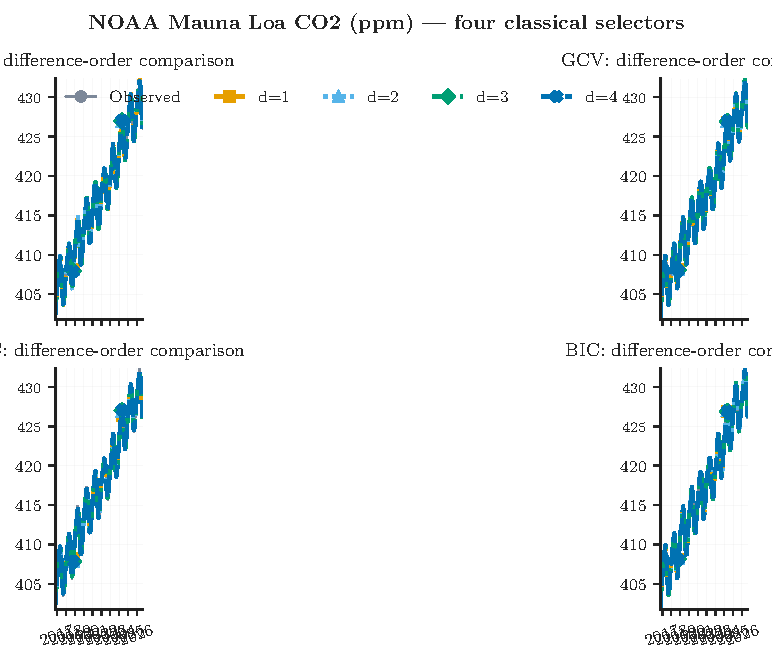
\includegraphics[width=\linewidth]{figures/co2_recent_criteria.pdf}
\caption{Sensitivity to the observation window: NOAA Mauna
Loa CO$_2$ over only the most recent 120 published months
with the same selection methods and difference orders
as Fig.~\ref{fig:co2-current-criteria}. Different windows
give different fitted problems and need not yield
the same selected normalized smoothness.}
\label{fig:co2-recent}
\end{figure}

The principal purpose of these comparisons is to expose
differences across \emph{selection methods, penalty orders,
sample periods and extrapolation conventions}, not to rank
future predictive ability from one observed realization.
A subsequent forecasting study should compare
multiple chronological origins and horizons, explicitly
account for seasonality and publication vintages, and
report paired loss differences with uncertainty.
